\chapter{Architectural Design}
\section{Overview}
This chapter focuses on the architectural structure, components will be described explaining how they interact with each other.
The system will be illustrated both physically and logically.

The main high level components of the system are the following:
\begin{description}
    \item[Application devices:] User devices where the application is installed. This application implements most of the logic of the system.
    \item[Cloud server:]  The server side of the system is responsible for the data storage and sync.
    
    This layer uses a NoSQL database, 
    which stores data in flexible, JSON-like, documents. The main keys are flexibility, expressive querying, realtime updates, offline support and scalability.
    \item[Web Application:] A pre-existing application used by administrators that allows to check and edit the stored data.
\end{description}

\newpage

\section{Component View}
\subsection{High-Level Component View}
\begin{figure}[!h]
    \centering
    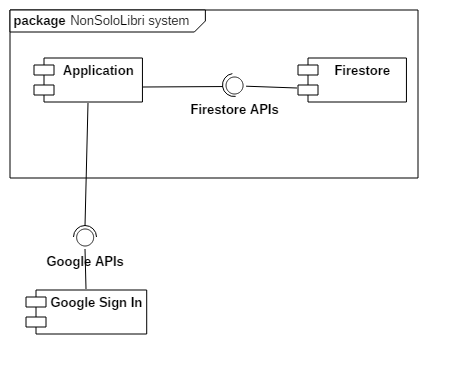
\includegraphics[scale=0.5]{images/high-level-component-view.png}
    \caption{High level component diagram}
    \label{ref:highlevelcomponentdiagram}
\end{figure}
This component diagram displays the high-level views of the system, focusing on application devices.

The components developed are:
\begin{description}
    \item[Application:] It is the core of the system, it manages all the information provided by the other services
     and performs the majority of the functions. It provides the client access to the entire system.
    \item[Firestore:] This component has account management and backup roles. It receives the data from the application and provides them when necessary.
\end{description}
Moreover, the application is integrated with \textbf{Google Sign In}, which provides the authentication functions of the system, 
using directly the credential of Google.
\clearpage
\subsection{Application}
\begin{figure}[!h]
    \centering
    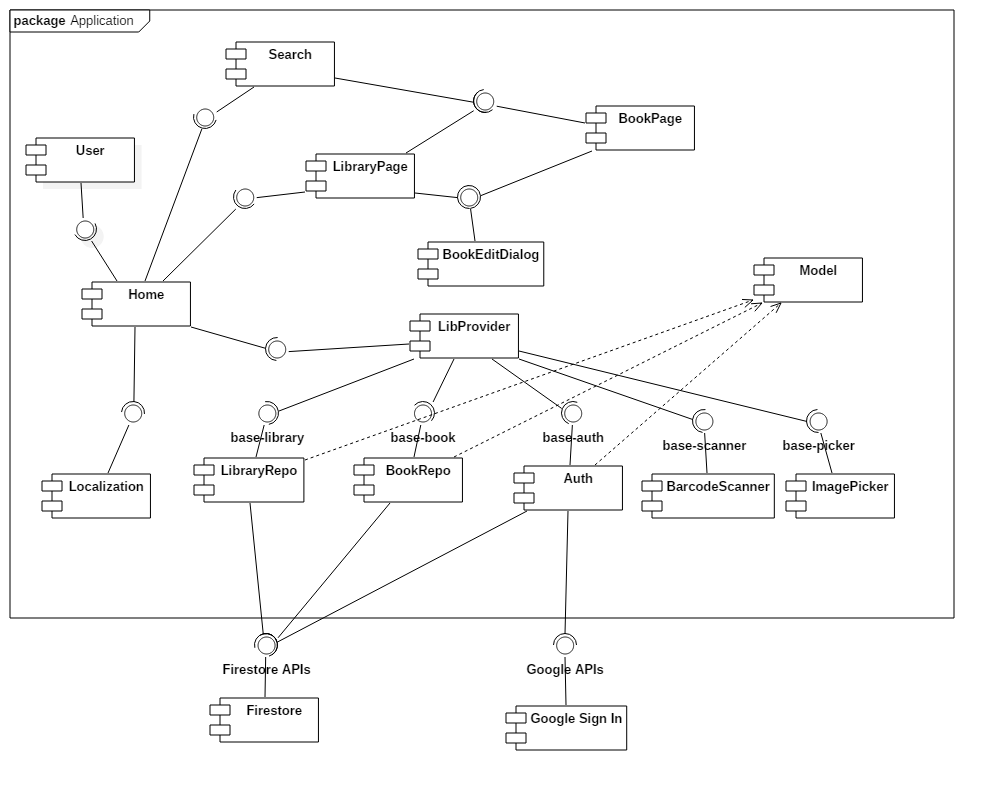
\includegraphics[scale=0.4]{images/application-component-diagram.png}
    \caption{Application component diagram}
    \label{ref:applicationcomponentdiagram}
\end{figure}
\begin{description}
    \item[Model:] It represents how data are structured in the application and ready to be stored by Firestore.
    \item[Home:] Is is the entry point of the application. Creates the Localization and LibProvider components. Handles login parts and the choice of the library.
    \item[Localization:] It sets up the language of the application based on the language of the OS.
    \item[LibProvider:] Provides LibraryRepo, BookRepo, Auth, BarcodeScanner and ImagePicker.
    \item[LibraryRepo:] This components is used to communicate with Firebase and to manage the library collection.
    \item[BookRepo:] It communicates with Firebase to save an retrieve books information.
    \item[Auth:] This components is used to handle the authentication of the user.
    \item[BarcodeScanner:] It uses the camera to read the ISBN from the barcode of a book.
    \item[ImagePicker:] It uses the library that allows to take a photo with camera or to pick an image from the gallery of the device.
    \item[LibraryPage:] It is a set of widgets that shows the books that belong to a given library.
    \item[BookPage:] It handles the information of the book, its reviews and the associated insertions made by other users. 
    \item[Search:] Shows a list of the books, which match with a user's input.
    \item[User:] It is the group of pages and widget that handles the profile management functionalities, including friendships and conversations between users.
\end{description}
\clearpage
\section{Relationship between the model and the database}
During the design of the application a database first approach was used. The database was the core during the design and the model was derived from it 
respecting the existing relationships between the entities.

The following is the ER diagram used to implement the database:
\begin{figure}[!h]
    \centering
    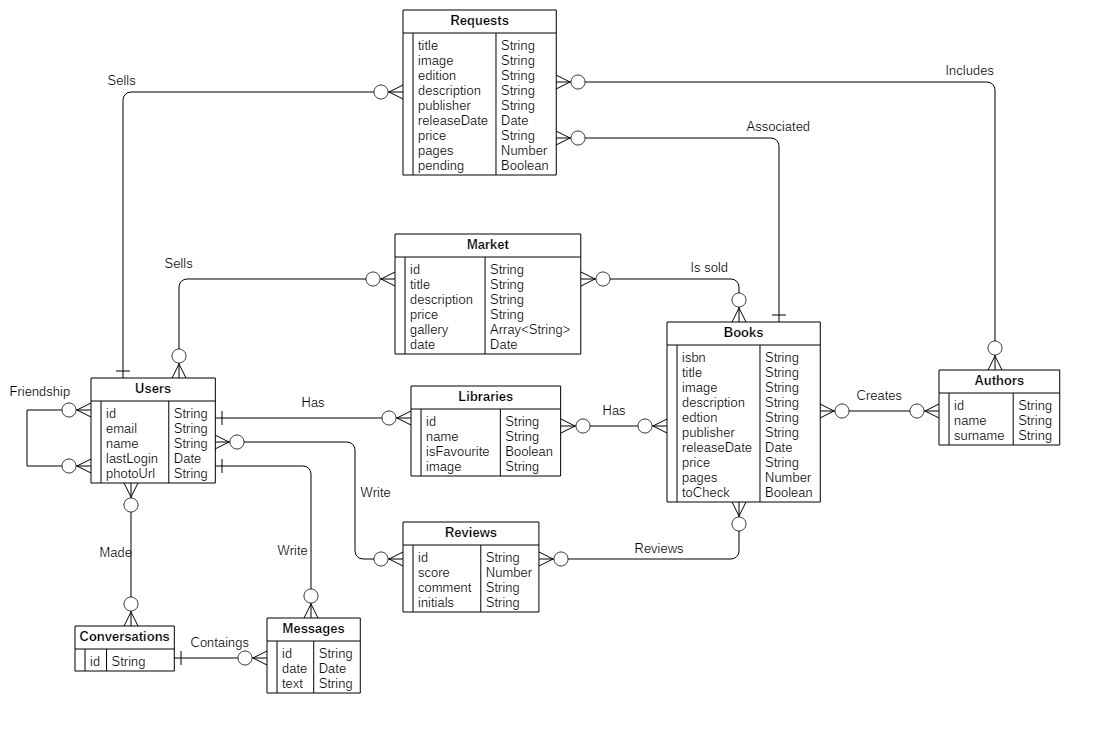
\includegraphics[scale=0.43]{images/er-diagram.png}
    \caption{ER diagram}
    \label{ref:erdiagram}
\end{figure}
\begin{description}
    \item[Books:] Collects all information of the books contained in the database. Each book is characterized  by a ISBN, which is its primary key, and other information including a title, a description and a image.
    \item[Users:] The users use the login function of the application. The id is generated automatically, the name and email are saved, but the password no.
    \item[Libraries:] The libraries created by each user.
    \item[Reviews:] Includes a score and a comment written by a user associated to a book.
    \item[Authors:] Contains the main information of the creator of one or more books.
    \item[Requests:] Contains all the suggestions made by a user to edit the book information. The idetifier is the union of the ISBN of the book and the user's id.
    \item[Market:] Collects the sales offers of books made by each user.
    \item[Conversations:] The discussion between two or more users.
    \item[Messages:] The texts exchanged during a conversation.
\end{description}
During the implementation, we opted for the introduction of data duplication. This allows to yield the main characteristics of the document-oriented database.
\clearpage
\subsection{Runtime View}
This section provides examples of how the main functionalities are implemented and their runtime behavior.
\subsubsection{Login}
\begin{figure}[!h]
    \centering
    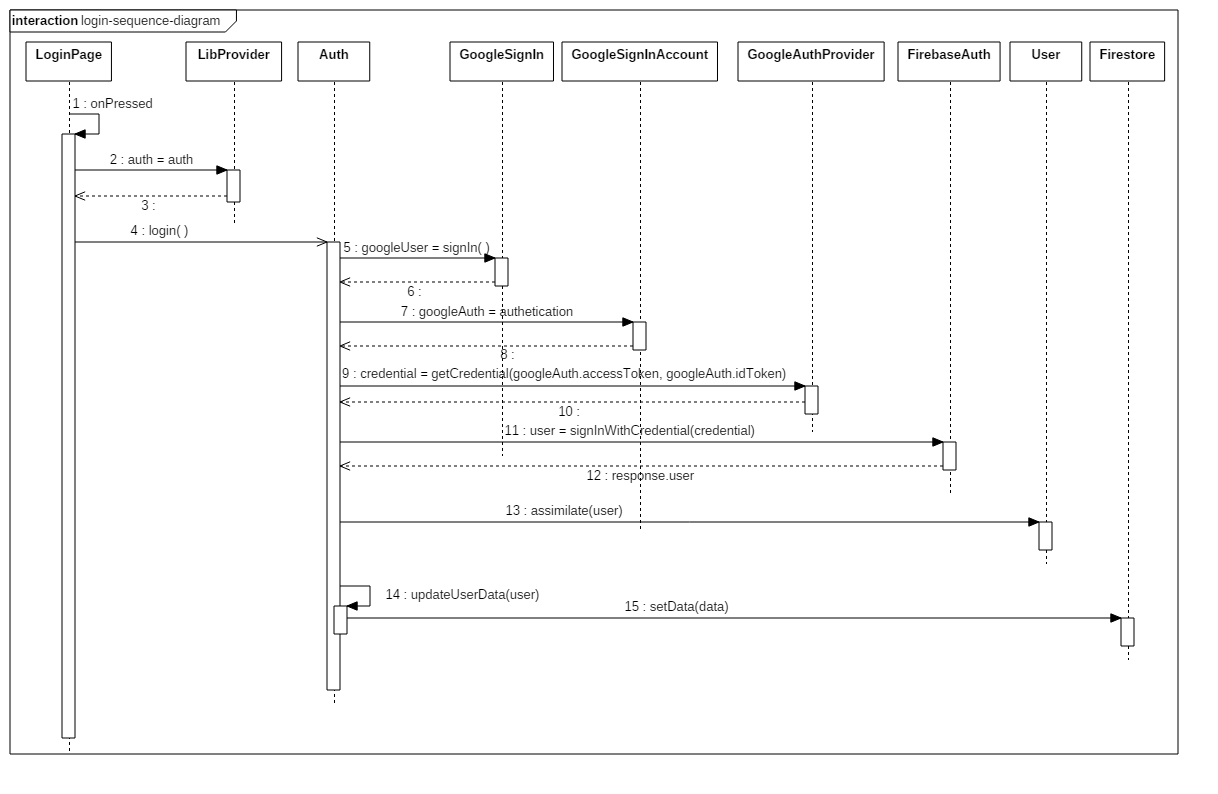
\includegraphics[scale=0.4]{images/login-sequence-diagram.png}
    \caption{Login sequence diagram}
    \label{ref:loginsequencediagram}
\end{figure}
The user taps the button on Login page, it retrieves the auth object from LibProvider. 
Auth handles the Google SignIn objects during the authentication phase and 
uses them to retrieve the user information (signInWithCredential.user).

Then, puts these information in a User object of the model using assimilate method and 
uses its updateUserDate method to save the user on Firestore.
\clearpage
\subsubsection{Add new book}
\begin{figure}[!h]
    \centering
    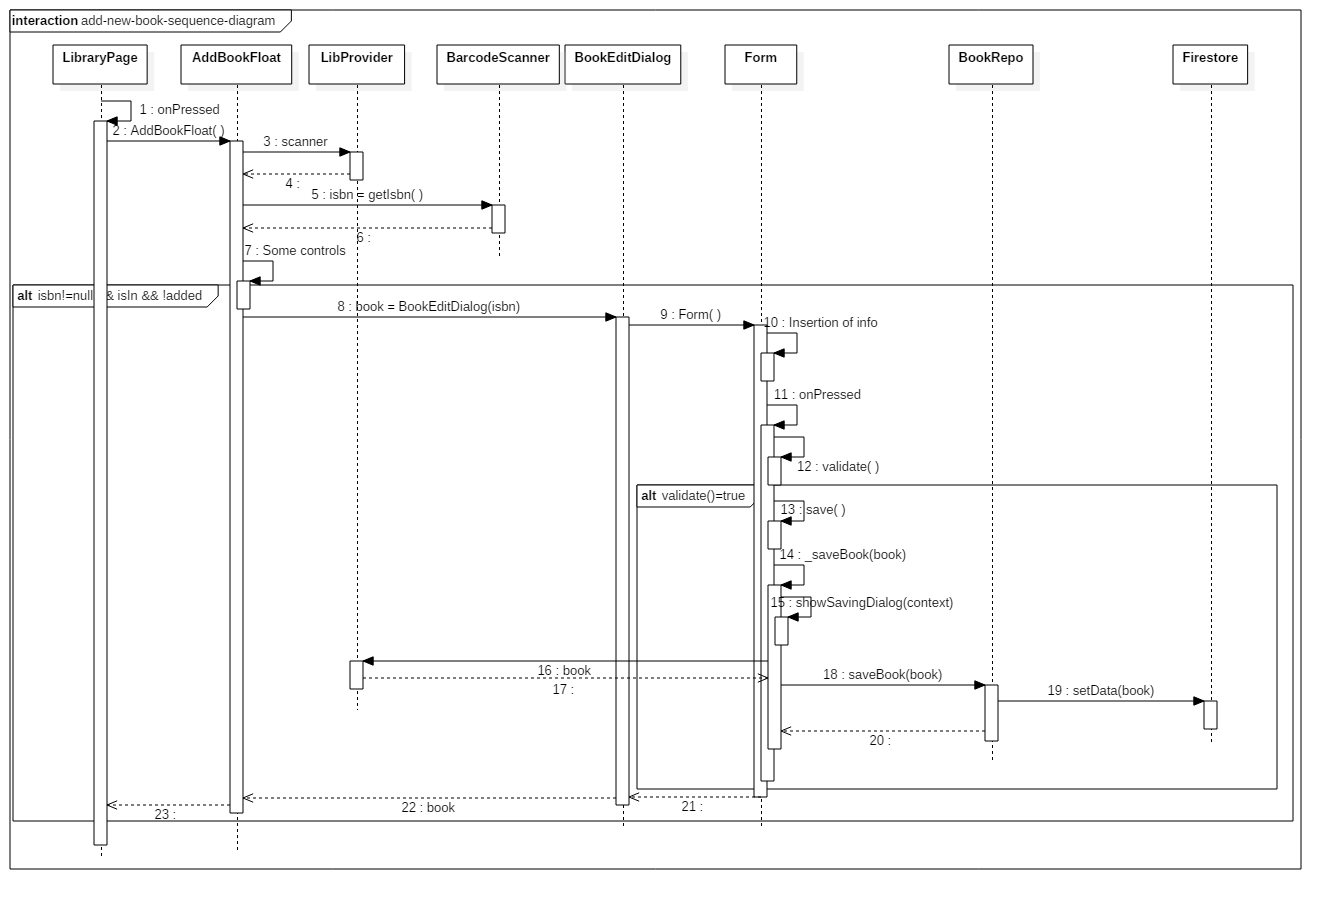
\includegraphics[scale=0.35]{images/add-new-book-sequence-diagram.png}
    \caption{Add new book sequence diagram}
    \label{ref:addnewbooksequencediagram}
\end{figure}
After the button of Library page is pressed, AddBookFloat is created and when tapped, it opens the camera by using the BarcodeScanner. 
The camera reads the ISBN, written in barcode form, and returns it to AddBookFloat.

AddBookFloat controls if the string returned is a valid ISBN, by using a regular expression, and if the book already exists. 
If it exists and is not already present in the library, adds it. If the book does not exists, the BookEditDialog is opened. 
This dialog contains a form and allows to type in the information of the book. 
When the insertion is finished, the button "done" is tapped and the form is validated and the information are saved 
Firestore using BookRepo. 